% Options for packages loaded elsewhere
\PassOptionsToPackage{unicode}{hyperref}
\PassOptionsToPackage{hyphens}{url}
\PassOptionsToPackage{dvipsnames,svgnames,x11names}{xcolor}
%
\documentclass[
]{article}

\usepackage{amsmath,amssymb}
\usepackage{iftex}
\ifPDFTeX
  \usepackage[T1]{fontenc}
  \usepackage[utf8]{inputenc}
  \usepackage{textcomp} % provide euro and other symbols
\else % if luatex or xetex
  \usepackage{unicode-math}
  \defaultfontfeatures{Scale=MatchLowercase}
  \defaultfontfeatures[\rmfamily]{Ligatures=TeX,Scale=1}
\fi
\usepackage{lmodern}
\ifPDFTeX\else  
    % xetex/luatex font selection
\fi
% Use upquote if available, for straight quotes in verbatim environments
\IfFileExists{upquote.sty}{\usepackage{upquote}}{}
\IfFileExists{microtype.sty}{% use microtype if available
  \usepackage[]{microtype}
  \UseMicrotypeSet[protrusion]{basicmath} % disable protrusion for tt fonts
}{}
\makeatletter
\@ifundefined{KOMAClassName}{% if non-KOMA class
  \IfFileExists{parskip.sty}{%
    \usepackage{parskip}
  }{% else
    \setlength{\parindent}{0pt}
    \setlength{\parskip}{6pt plus 2pt minus 1pt}}
}{% if KOMA class
  \KOMAoptions{parskip=half}}
\makeatother
\usepackage{xcolor}
\setlength{\emergencystretch}{3em} % prevent overfull lines
\setcounter{secnumdepth}{5}
% Make \paragraph and \subparagraph free-standing
\ifx\paragraph\undefined\else
  \let\oldparagraph\paragraph
  \renewcommand{\paragraph}[1]{\oldparagraph{#1}\mbox{}}
\fi
\ifx\subparagraph\undefined\else
  \let\oldsubparagraph\subparagraph
  \renewcommand{\subparagraph}[1]{\oldsubparagraph{#1}\mbox{}}
\fi


\providecommand{\tightlist}{%
  \setlength{\itemsep}{0pt}\setlength{\parskip}{0pt}}\usepackage{longtable,booktabs,array}
\usepackage{calc} % for calculating minipage widths
% Correct order of tables after \paragraph or \subparagraph
\usepackage{etoolbox}
\makeatletter
\patchcmd\longtable{\par}{\if@noskipsec\mbox{}\fi\par}{}{}
\makeatother
% Allow footnotes in longtable head/foot
\IfFileExists{footnotehyper.sty}{\usepackage{footnotehyper}}{\usepackage{footnote}}
\makesavenoteenv{longtable}
\usepackage{graphicx}
\makeatletter
\def\maxwidth{\ifdim\Gin@nat@width>\linewidth\linewidth\else\Gin@nat@width\fi}
\def\maxheight{\ifdim\Gin@nat@height>\textheight\textheight\else\Gin@nat@height\fi}
\makeatother
% Scale images if necessary, so that they will not overflow the page
% margins by default, and it is still possible to overwrite the defaults
% using explicit options in \includegraphics[width, height, ...]{}
\setkeys{Gin}{width=\maxwidth,height=\maxheight,keepaspectratio}
% Set default figure placement to htbp
\makeatletter
\def\fps@figure{htbp}
\makeatother
\newlength{\cslhangindent}
\setlength{\cslhangindent}{1.5em}
\newlength{\csllabelwidth}
\setlength{\csllabelwidth}{3em}
\newlength{\cslentryspacingunit} % times entry-spacing
\setlength{\cslentryspacingunit}{\parskip}
\newenvironment{CSLReferences}[2] % #1 hanging-ident, #2 entry spacing
 {% don't indent paragraphs
  \setlength{\parindent}{0pt}
  % turn on hanging indent if param 1 is 1
  \ifodd #1
  \let\oldpar\par
  \def\par{\hangindent=\cslhangindent\oldpar}
  \fi
  % set entry spacing
  \setlength{\parskip}{#2\cslentryspacingunit}
 }%
 {}
\usepackage{calc}
\newcommand{\CSLBlock}[1]{#1\hfill\break}
\newcommand{\CSLLeftMargin}[1]{\parbox[t]{\csllabelwidth}{#1}}
\newcommand{\CSLRightInline}[1]{\parbox[t]{\linewidth - \csllabelwidth}{#1}\break}
\newcommand{\CSLIndent}[1]{\hspace{\cslhangindent}#1}

\makeatletter
\makeatother
\makeatletter
\makeatother
\makeatletter
\@ifpackageloaded{caption}{}{\usepackage{caption}}
\AtBeginDocument{%
\ifdefined\contentsname
  \renewcommand*\contentsname{Table of contents}
\else
  \newcommand\contentsname{Table of contents}
\fi
\ifdefined\listfigurename
  \renewcommand*\listfigurename{List of Figures}
\else
  \newcommand\listfigurename{List of Figures}
\fi
\ifdefined\listtablename
  \renewcommand*\listtablename{List of Tables}
\else
  \newcommand\listtablename{List of Tables}
\fi
\ifdefined\figurename
  \renewcommand*\figurename{Figure}
\else
  \newcommand\figurename{Figure}
\fi
\ifdefined\tablename
  \renewcommand*\tablename{Table}
\else
  \newcommand\tablename{Table}
\fi
}
\@ifpackageloaded{float}{}{\usepackage{float}}
\floatstyle{ruled}
\@ifundefined{c@chapter}{\newfloat{codelisting}{h}{lop}}{\newfloat{codelisting}{h}{lop}[chapter]}
\floatname{codelisting}{Listing}
\newcommand*\listoflistings{\listof{codelisting}{List of Listings}}
\makeatother
\makeatletter
\@ifpackageloaded{caption}{}{\usepackage{caption}}
\@ifpackageloaded{subcaption}{}{\usepackage{subcaption}}
\makeatother
\makeatletter
\@ifpackageloaded{tcolorbox}{}{\usepackage[skins,breakable]{tcolorbox}}
\makeatother
\makeatletter
\@ifundefined{shadecolor}{\definecolor{shadecolor}{rgb}{.97, .97, .97}}
\makeatother
\makeatletter
\makeatother
\makeatletter
\makeatother
\ifLuaTeX
  \usepackage{selnolig}  % disable illegal ligatures
\fi
\IfFileExists{bookmark.sty}{\usepackage{bookmark}}{\usepackage{hyperref}}
\IfFileExists{xurl.sty}{\usepackage{xurl}}{} % add URL line breaks if available
\urlstyle{same} % disable monospaced font for URLs
\hypersetup{
  pdftitle={Note 1},
  pdfauthor={Hans Martinez},
  colorlinks=true,
  linkcolor={blue},
  filecolor={Maroon},
  citecolor={Blue},
  urlcolor={Blue},
  pdfcreator={LaTeX via pandoc}}

\title{Note 1}
\author{Hans Martinez}
\date{2024-01-19}

\begin{document}
\maketitle
\ifdefined\Shaded\renewenvironment{Shaded}{\begin{tcolorbox}[sharp corners, boxrule=0pt, borderline west={3pt}{0pt}{shadecolor}, enhanced, interior hidden, frame hidden, breakable]}{\end{tcolorbox}}\fi

\hypertarget{profit-maximizationsource}{%
\section[Profit Maximization]{\texorpdfstring{Profit
Maximization\footnote{Example and figures taken from Varian (2014)}}{Profit Maximization}}\label{profit-maximizationsource}}

Let \(y=f(x)\) be the production function of a firm. The firm faces
output prices \(p\), and the price of the input \(w\). The
profit-maximization problem facing the firm can be written as

\[
\max_x pf(x)-wx
\]

\hypertarget{revealed-profitability}{%
\section{Revealed Profitability}\label{revealed-profitability}}

When a profit-maximizing firm makes its choice of inputs and outputs it
reveals two things:

\begin{enumerate}
\def\labelenumi{\arabic{enumi}.}
\tightlist
\item
  \emph{feasible} production plan
\item
  these choices are more profitable than other feasible choices that the
  firm could have made
\end{enumerate}

Suppose you observe two choices that the firm makes at two different
sets of prices. At time \(t\), it faces \((p^t,w^t)\) and makes choices
\((y^t,x^t)\). At time \(s\), it faces prices \((p^s,w^s)\) and makes
choices \((y^s,x^s)\). If the production function of the firms hasn't
changed from times \(s\) and \(t\) and if the firm is a profit
maximizer, then we must have

\begin{equation}\protect\hypertarget{eq-rev-prof-t}{}{
p^ty^t-w^tx^t\ge p^ty^s-w^tx^s
}\label{eq-rev-prof-t}\end{equation}

and

\begin{equation}\protect\hypertarget{eq-rev-prof-s}{}{
p^sy^s-w^sx^s\ge p^sy^t-w^sx^t
}\label{eq-rev-prof-s}\end{equation}

In other words, the profits that the firm achieved facing the \(t\)
period prices must be larger than if they used the \(s\) period plan and
vice versa.

If either of these inequalities were violated, the firm could not have
been a profit-maximizer (with an unchanging technology).

The satisfaction of these inequalities might be referred to as the
\textbf{Weak Axiom of Profit Maximization (WAPM)}.

These inequalities provide a practical test for the profit-maximization
model. In other words, if the inequalities are met we cannot reject the
hypothesis that firms are profit-maximizers under unchanging technology
and price-taking behavior.

In addition, if the firm's choices satisfy WAPM, we can derive a useful
comparative statics statement about the behavior of factor demand and
output supplies when prices change. Transpose the two sides of
Equation~\ref{eq-rev-prof-s} to get

\begin{equation}\protect\hypertarget{eq-rev-prof-s-trans}{}{
-p^sy^t+w^sx^t\ge -p^sy^s+w^sx^s
}\label{eq-rev-prof-s-trans}\end{equation}

and add Equation~\ref{eq-rev-prof-s-trans} to
Equation~\ref{eq-rev-prof-t} to get

\begin{equation}\protect\hypertarget{eq-rev-prof-both}{}{
\begin{aligned}
(p^t-p^s)y^t-(w^t-w^s)x^t \ge (p^t-p^s)y^s-(w^t-w^s)x^s
\end{aligned}
}\label{eq-rev-prof-both}\end{equation}

Rearrange to get

\begin{equation}\protect\hypertarget{eq-rev-prof}{}{
(p^t-p^s)(y^t-y^s)-(w^t-w^s)(x^t-x^s) \ge 0
}\label{eq-rev-prof}\end{equation}

Finally, define change in prices, \(\Delta p=(p^t-p^s)\), change in
output \(\Delta y = (y^t-y^s)\), and so on

\begin{equation}\protect\hypertarget{eq-rev-prof-Delta}{}{
\Delta p \Delta y - \Delta w \Delta x \ge 0
}\label{eq-rev-prof-Delta}\end{equation}

Our final result says that the change in the price of output times the
change in output minus the change in the price of input times the change
in the input must be non-negative. This equation contains all the
comparative statics results about profit maximization.

For example, suppose the price of output changes but the price of the
input stays constant. Then, because \(\Delta w = 0\),
Equation~\ref{eq-rev-prof-Delta} reduces to

\begin{equation}\protect\hypertarget{eq-rev-prof-Delta-noinput}{}{
\Delta p \Delta y \ge 0
}\label{eq-rev-prof-Delta-noinput}\end{equation}

Therefore, if the price of output increases, \(\Delta p \ge 0\), then
the change in output must be non-negative as well, \(\Delta y \ge 0\).
This says that the profit-maximizing supply curve of a competitive firm
must have a positive (or at least zero) slope.

Similarly, if the price of the output remains constant,
Equation~\ref{eq-rev-prof-Delta} becomes

\begin{equation}\protect\hypertarget{eq-rev-prof-Delta-nooutput}{}{
\begin{aligned}
 - \Delta w \Delta x &\ge 0 \\
\Delta w \Delta x &\le 0
\end{aligned}
}\label{eq-rev-prof-Delta-nooutput}\end{equation}

Thus if the price of the input goes up, \(\Delta w \ge 0\), then the
demand for the input will go down (or at least remain the same),
\(\Delta x \le 0\). This means that the factor demand curve must be a
decreasing function of the input prices: input demand curves have a
negative slope.

If we observe a firm's choices, and these choices satisfy WAPM, we can
construct an estimate of the technology for which the observed choices
are profit-maximizing choices.

Suppose we are given an observed choice in period \(t\) and \(s\), as
above.

\begin{enumerate}
\def\labelenumi{\arabic{enumi}.}
\tightlist
\item
  Calculate the profits \(\pi_s\) and \(\pi_t\) and plot all the
  combinations of \(y\) and \(x\) that yield these profits.
\end{enumerate}

\[
\begin{aligned}
\pi_t&=p^ty-w^tx \\
\pi_s&=p^sy-w^sx
\end{aligned}
\]

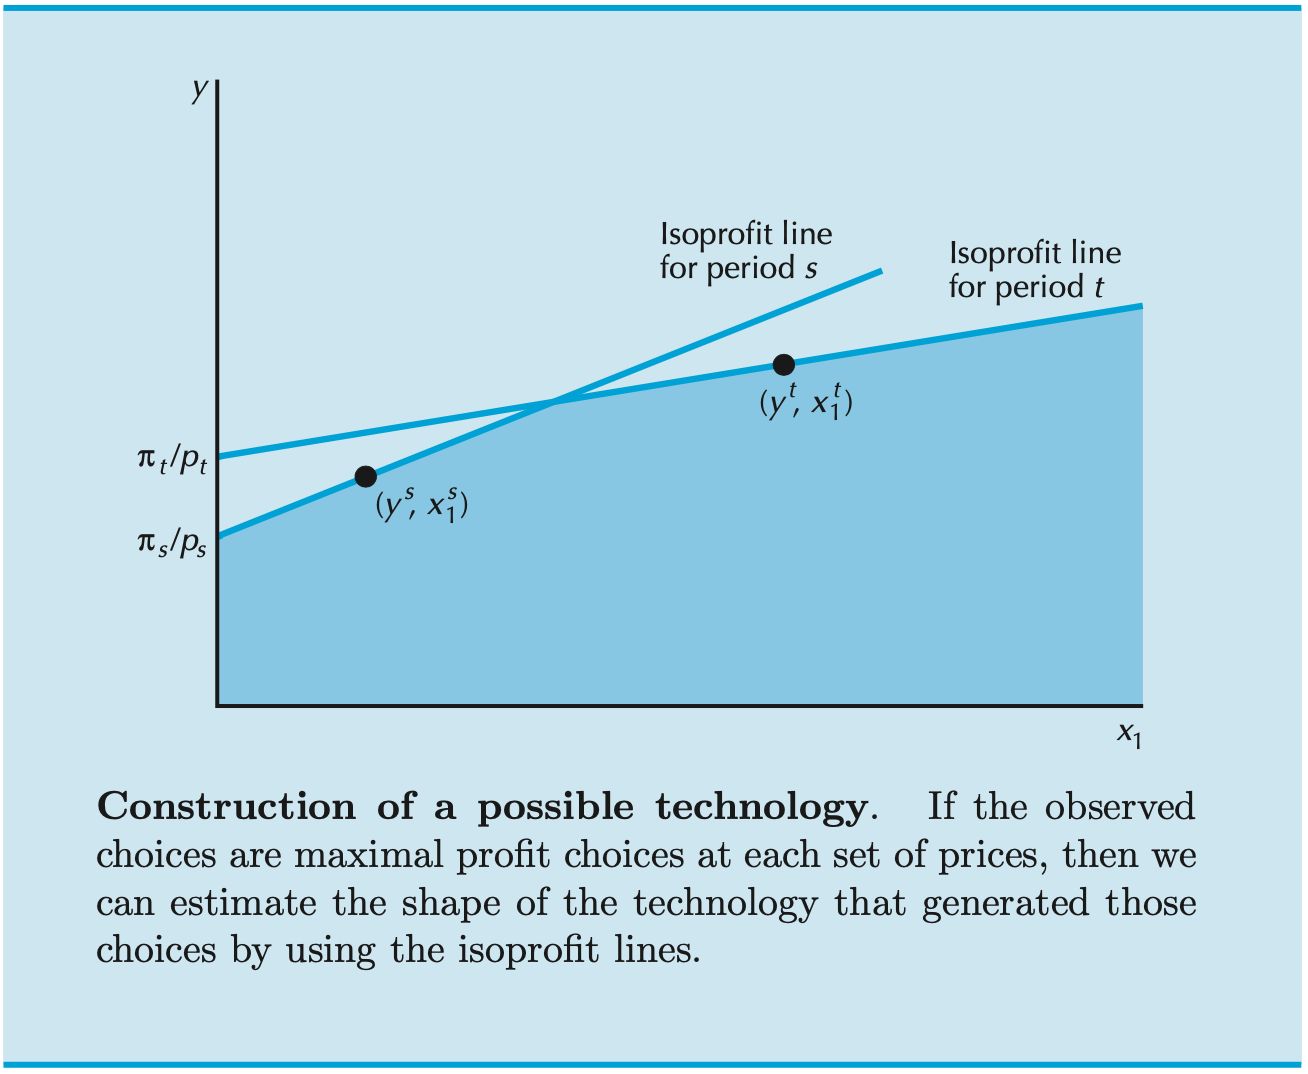
\includegraphics{figures/rev_prof__2.png}

The points above the isoprofit line for period \(t\) represent higher
profits than \(\pi_t\) at period \(t\) prices, the points above the
isoprofit line for period \(s\) represent higher profits than \(\pi_s\)
at period \(s\) prices.

WAPM requires that the choice in period \(t\) must lie below the period
\(s\) isoprofit line and that the choice in period \(s\) must lie below
the period \(t\) isoprofit line.

If this condition is satisfied, the shaded area beneath the two lines
approximates the technology for which \((y^t, x^t)\) and \((y^s, x^s)\)
are profit-maximizing choices.

The proof that this technology will generate the observed choices as
profit-maximizing choices is clear geometrically. At the prices
\((p^t , w^t )\), the choice \((y^t,x^t)\) is on the highest isoprofit
line possible, and the same goes for the period \(s\) choice.

Thus, when the observed choices satisfy WAPM, we can ``reconstruct'' an
estimate of a technology that might have generated the observations. In
this sense, any observed choices consistent with WAPM could be profit-
maximizing choices. As we observe more choices that the firm makes, we
get a tighter estimate of the production function.

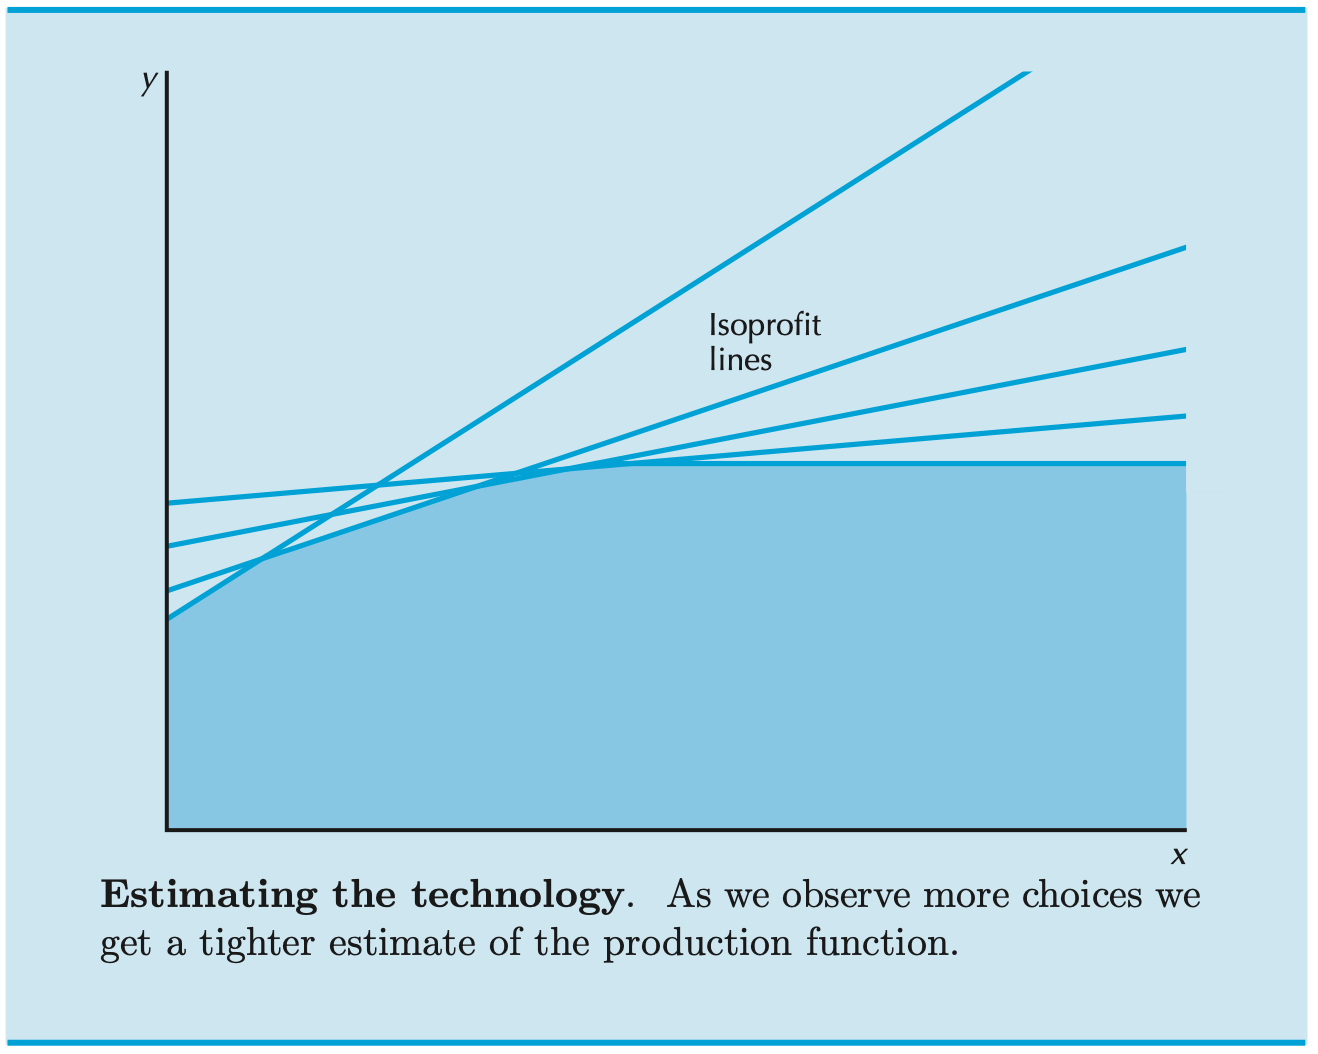
\includegraphics{figures/rev_prof_n.png}

This estimate of the production function can be used to forecast firm
behavior in other environments or for other uses in economic analysis.

\hypertarget{references}{%
\subsection*{References}\label{references}}
\addcontentsline{toc}{subsection}{References}

\hypertarget{refs}{}
\begin{CSLReferences}{1}{0}
\leavevmode\vadjust pre{\hypertarget{ref-Varian2014}{}}%
Varian, Hal R. 2014. \emph{Intermediate Microeconomics with Calculus}.
NY: W.W. Norton; Company.

\end{CSLReferences}



\end{document}
